\chapter{MVP}\label{chap:mvp}

En este capítulo se presenta la transición de la propuesta desde un prototipo funcional hacia un producto mínimo viable. Mientras que el prototipo estuvo orientado principalmente a validar la factibilidad técnica de la extracción automática de información desde carátulas bancarias, el MVP amplía dicho alcance hacia una arquitectura más general basada en extractores configurables. En este enfoque, la información a extraer se define mediante \textit{schemas}, \textit{prompts} y modelos, lo que permite adaptar el sistema a distintos tipos de documentos. La Tabla \ref{tab:proto_vs_mvp} resume las diferencias principales entre ambas etapas.

\begin{table}[H]
\centering
\resizebox{0.9\textwidth}{!}{%
\begin{tabular}{l l l}
\toprule
\textbf{Aspecto} & \textbf{Prototipo} & \textbf{MVP} \\
\midrule
Objetivo & Validar factibilidad técnica & Generar valor operativo \\
Tipo de datos & \textit{Dataset} controlado & Documentos reales \\
Extracción & Ejecución aislada & Integrada en \textit{pipeline} \\
Validación & Limitada & Validación estructural + humana \\
Persistencia & SQLite local & Base de datos (PostgreSQL) \\
Interacción usuario & No considerada & Revisión y corrección \\
Métricas & Evaluación \textit{offline} & Monitoreo en tiempo real \\
Escalabilidad & No considerada & Modular y extensible \\
\bottomrule
\end{tabular}
}
\caption{Comparación entre prototipo y MVP}
\label{tab:proto_vs_mvp}
\end{table}


\section{Objetivo del MVP}

El objetivo del MVP es ofrecer una versión mínima operativa de la solución capaz de integrarse en flujos de \textit{onboarding} para automatizar la captura y validación inicial de información contenida en documentos. A diferencia del prototipo, el sistema no se limita a un único tipo de documento, sino que permite definir extractores configurables mediante \textit{schemas} que especifican los campos a extraer, junto con \textit{prompts} y modelos asociados, lo que habilita la adaptación del sistema a distintos escenarios de validación de documentos. Esta decisión de diseño surge directamente de los hallazgos experimentales descritos en el capítulo anterior, donde se observó que la precisión de la extracción varía significativamente según el formato del documento y la institución bancaria de origen. En lugar de intentar construir un extractor monolítico que cubra todos los casos posibles, el MVP delega la especialización al usuario, proporcionando herramientas de asistencia basadas en inteligencia artificial para la generación de schemas y prompts, así como mecanismos de evaluación mediante extracciones de prueba con resultados visibles. De esta manera, el sistema puede evolucionar su cobertura sin requerir modificaciones en el código fuente, ya que cada nuevo tipo de documento se incorpora como una configuración adicional.



\section{Usuario objetivo del MVP}

El sistema contempla tres perfiles de usuario con distintos niveles de acceso. El perfil principal corresponde al usuario operativo, encargado de registrar o validar información bancaria dentro del proceso de \textit{onboarding}, cuya función consiste en cargar documentos, revisar la información extraída y confirmar o corregir campos clave como el titular de la cuenta, el banco y el número CLABE; este perfil no requiere conocimientos técnicos especializados, ya que la interfaz presenta los datos de forma editable y guía al usuario a lo largo del flujo de validación. El segundo perfil es el administrador, quien tiene la capacidad de gestionar usuarios (crear, editar roles, activar o desactivar cuentas), configurar extractores y acceder a métricas de precisión agregadas a través de un \textit{dashboard}. El tercer perfil corresponde al usuario invitado (\textit{guest}), que se asigna automáticamente a cualquier persona que inicie sesión por primera vez mediante GitHub OAuth y opera bajo límites diarios de uso: 10 extracciones, 1 extractor configurable y 10 llamadas al asistente de inteligencia artificial por día, lo que permite que usuarios externos exploren la funcionalidad del sistema sin comprometer los recursos de procesamiento. Adicionalmente, el sistema ofrece tokens de API para acceso programático, lo que habilita la integración con sistemas externos sin necesidad de interactuar con la interfaz web.


\section{Alcance funcional del MVP}

El producto mínimo viable incorpora un enfoque basado en extractores configurables, donde cada tipo de documento se define mediante un \textit{schema} JSON que especifica los campos requeridos, un \textit{prompt} de extracción en lenguaje natural y un modelo de lenguaje asociado, lo que permite que el sistema no dependa de lógica fija para un único documento, sino que pueda adaptarse dinámicamente a distintos formatos mediante la configuración de nuevos extractores. La creación de un extractor se realiza a través de un asistente guiado de cuatro pasos: primero, el usuario define el nombre, la descripción y el modelo a utilizar; segundo, construye el \textit{schema} de salida con los campos que el sistema debe extraer del documento, donde un asistente de inteligencia artificial puede generar el \textit{schema} automáticamente a partir de una descripción en lenguaje natural; tercero, redacta o genera el \textit{prompt} de extracción, con la posibilidad de refinarlo iterativamente mediante instrucciones adicionales procesadas por el mismo asistente; y cuarto, opcionalmente realiza una extracción de prueba sobre un documento real para verificar que la configuración produce los resultados esperados antes de activar el extractor.

El sistema también incorpora un mecanismo de versionamiento que permite crear variantes de un mismo extractor con diferentes \textit{prompts} o modelos. Cuando existen versiones activas, el sistema selecciona aleatoriamente entre la configuración base y las variantes durante cada extracción, registrando en los \textit{logs} cuál fue utilizada, lo que habilita la comparación empírica entre configuraciones sobre documentos reales y proporciona datos objetivos para decidir cuál variante ofrece mejores resultados en producción. Complementariamente, un \textit{dashboard} de métricas permite observar la tasa de correcciones por campo y por extractor, ofreciendo visibilidad continua sobre la precisión del sistema e identificando oportunidades de mejora.

\section{Elementos fuera de alcance}

Si bien el MVP amplía el alcance del prototipo mediante extractores configurables que permiten adaptar el sistema a distintos tipos de documentos, todavía constituye una versión acotada del producto. En particular, no contempla validación en tiempo real contra APIs bancarias para verificar si una CLABE existe o se encuentra activa, ni incorpora mecanismos de detección de fraude, falsificación documental o análisis de autenticidad de imágenes. De igual manera, quedan fuera de su alcance los documentos manuscritos o aquellos cuya legibilidad no cumpla con condiciones mínimas de procesamiento, así como el mecanismo de \textit{retry} automático evaluado durante los experimentos. En cuanto a la capa de monitoreo, el \textit{dashboard} se limita por ahora a la visualización básica de métricas agregadas, sin filtros avanzados, exportación, alertas personalizadas o análisis detallado por banco o periodo. En conjunto, estas exclusiones permiten mantener una delimitación clara del MVP y concentrar el desarrollo en el flujo mínimo que genera valor operacional.

\section{Supuestos críticos}

El diseño del MVP se sustenta en un conjunto de supuestos que, de no cumplirse, podrían comprometer la viabilidad o el impacto de la solución. La Tabla~\ref{tab:supuestos_criticos} formaliza estos supuestos junto con su criticidad y las consecuencias en caso de resultar falsos. Su explicitación permite identificar de forma anticipada los puntos donde el sistema es más vulnerable y orienta las prioridades de validación durante la operación inicial.

\begin{table}[H]
\centering
\resizebox{\textwidth}{!}{%
\begin{tabular}{p{5cm} p{4.5cm} p{5cm}}
\toprule
\textbf{Supuesto} & \textbf{Por qué es crítico} & \textbf{Consecuencia si es falso} \\
\midrule
Los \textit{LLMs} con un \textit{prompt} adecuado pueden manejar la variedad de formatos y calidades de documentos bancarios & El sistema depende de la capacidad del modelo para interpretar documentos no vistos durante la experimentación & La precisión se degrada con formatos nuevos y el sistema requiere ajustes constantes de \textit{prompts} por banco \\
El sistema puede extenderse a otros tipos de documentos financieros mediante extractores configurables & Limita el valor a largo plazo si solo funciona para carátulas bancarias & Se requiere reimplementación específica para cada nuevo tipo de documento \\
Los usuarios confiarán en los datos pre-completados y corregirán cuando sea necesario & Sin adopción no hay reducción real de la carga operativa de soporte & El sistema no genera impacto operativo y la \textit{fintech} mantiene el flujo manual \\
El costo por llamada a la API de Claude se mantiene viable a escala & El procesamiento por documento es el costo variable principal del sistema & A volúmenes altos el costo unitario supera el valor generado, comprometiendo la sostenibilidad económica \\
\bottomrule
\end{tabular}
}
\caption{Supuestos críticos del MVP}
\label{tab:supuestos_criticos}
\end{table}

\section{Arquitectura mínima operable}

La arquitectura del MVP se estructura en cinco componentes principales: la interfaz de usuario, el \textit{backend} de procesamiento, la capa de extracción basada en modelos de lenguaje, la persistencia de resultados y el almacenamiento de documentos. La interfaz de usuario constituye el punto de interacción con la solución, permitiendo la carga de carátulas bancarias, la visualización de la información extraída y la validación o corrección de los resultados por parte del usuario. El \textit{backend}, implementado en \textit{FastAPI}, actúa como orquestador del flujo completo de carga, procesamiento, validación y respuesta. Sobre esta capa operan extractores configurables que encapsulan la lógica de extracción mediante la definición de \textit{schemas}, \textit{prompts} y modelos asociados. Este diseño permite desacoplar la lógica de extracción del tipo de documento, facilitando la incorporación de nuevos casos sin modificar el \textit{pipeline} principal, cuya salida se traduce en un JSON estructurado con campos validados y metadatos de extracción. Desde el punto de vista de infraestructura, el despliegue mínimo operable se apoya en Railway como plataforma de ejecución, \textit{PostgreSQL} como base de datos para la persistencia de resultados y un servicio de almacenamiento compatible con S3 proporcionado por Railway para el almacenamiento de documentos. Esta arquitectura permite separar responsabilidades, mantener trazabilidad y sostener una operación básica de punta a punta. Los enlaces al repositorio, la aplicación desplegada y la documentación de la API se encuentran disponibles en el Apéndice~\ref{apendice:recursos}. Asimismo, la solución adopta un esquema semiautomatizado, en el que el sistema realiza la extracción inicial y genera señales de confianza, mientras que el usuario interviene en la validación final antes del almacenamiento definitivo. La Figura \ref{fig:layers_architecture} ilustra la organización en capas del sistema, mientras que la Figura \ref{fig:infra_mvp} muestra los componentes de infraestructura y sus interacciones.




\begin{figure}[H]
\centering
\resizebox{0.55\textwidth}{!}{
\begin{tikzpicture}[
    node distance=1.2cm,
    every node/.style={font=\small, align=center},
    capa/.style={
        rectangle, rounded corners=6pt, draw=gray!40, thick,
        minimum width=12cm, minimum height=2.2cm, fill=white
    },
    componente/.style={
        rectangle, rounded corners=4pt, thick,
        minimum width=3.4cm, minimum height=1.0cm
    },
    flecha/.style={-{Latex[length=3mm]}, thick}
]

% === CAPA 1: Cliente ===
\node[capa, minimum height=2.6cm] (c1) {};
\node[font=\footnotesize\scshape, text=gray!60, anchor=north] at ([yshift=-0.1cm]c1.north) {Cliente};
\node[componente, draw=gray!50, fill=gray!8] at ([yshift=-0.2cm]c1.center) {Web UI (\textit{Upload} / \textit{Review} / \textit{Confirm})};

% === CAPA 2: API Layer ===
\node[capa, below=of c1, minimum height=3.2cm] (c2) {};
\node[font=\footnotesize\scshape, text=gray!60, anchor=north] at ([yshift=-0.1cm]c2.north) {API \textit{Layer}};
\node[componente, draw=teal!40, fill=teal!8, text width=5.5cm] at ([yshift=-0.2cm]c2.center) {
    FastAPI REST API\\[1pt]
    {\scriptsize \textit{Upload Endpoint}}\\
    {\scriptsize \textit{Extraction Endpoint} $\cdot$ \textit{Results Endpoint}}
};

% === CAPA 3: Procesamiento ===
\node[capa, below=of c2, minimum height=3.0cm] (c3) {};
\node[font=\footnotesize\scshape, text=gray!60, anchor=north] at ([yshift=-0.1cm]c3.north) {Capa de procesamiento};
\node[componente, draw=orange!40, fill=orange!8] at ([xshift=-3.8cm, yshift=-0.2cm]c3.center) {
    \textit{LLM Orchestration}\\[1pt]{\scriptsize \textit{Prompts} + \textit{routing}}
};
\node[componente, draw=orange!40, fill=orange!8] at ([yshift=-0.2cm]c3.center) {
    \textit{Parser Registry}\\[1pt]{\scriptsize \textit{Configs} + versiones}
};
\node[componente, draw=orange!40, fill=orange!8] at ([xshift=3.8cm, yshift=-0.2cm]c3.center) {
    \textit{Schema Validation}\\[1pt]{\scriptsize CLABE + \textit{retry}}
};

% === CAPA 4: Persistencia ===
\node[capa, below=of c3, minimum height=3.6cm] (c4) {};
\node[font=\footnotesize\scshape, text=gray!60, anchor=north] at ([yshift=-0.1cm]c4.north) {Persistencia \& servicios externos};
\node[componente, draw=teal!40, fill=teal!8, text width=3cm] at ([xshift=-3.8cm, yshift=-0.2cm]c4.center) {
    PostgreSQL\\[1pt]{\scriptsize \textit{Schemas}}\\{\scriptsize \textit{Results}}\\{\scriptsize \textit{Metadata}}
};
\node[componente, draw=orange!30, fill=orange!5, text width=3cm] at ([yshift=-0.2cm]c4.center) {
    Railway \textit{Buckets}\\[1pt]{\scriptsize \textit{Images}}\\{\scriptsize \textit{Documents}}
};
\node[componente, draw=teal!30, fill=teal!5, text width=3cm] at ([xshift=3.8cm, yshift=-0.2cm]c4.center) {
    \textit{LLM} APIs\\[1pt]{\scriptsize Claude}\\{\scriptsize GPT-4}\\{\scriptsize Gemini}
};

% === Flechas entre capas ===
\draw[flecha] (c1.south) -- (c2.north);
\draw[flecha] (c2.south) -- (c3.north);
\draw[flecha] (c3.south) -- (c4.north);

\end{tikzpicture}
}
\caption{Arquitectura en capas del MVP}
\label{fig:layers_architecture}
\end{figure}

\begin{figure}[H]
\centering
\resizebox{0.7\textwidth}{!}{
\begin{tikzpicture}[
    node distance=1.2cm and 2cm,
    every node/.style={font=\small, align=center},
    servicio/.style={
        rectangle, rounded corners=6pt, thick,
        minimum width=3.5cm, minimum height=1.6cm
    },
    plataforma/.style={
        rectangle, rounded corners=6pt, draw=gray!40, dashed, thick,
        inner sep=14pt
    },
    etiqueta/.style={font=\scriptsize\itshape, text=gray!60},
    flecha/.style={-{Latex[length=3mm]}, thick}
]

% === Servicios internos ===
\node[servicio, draw=teal!40, fill=teal!8] (fastapi) {
    FastAPI\\[1pt]{\scriptsize \textit{Backend} API}
};
\node[servicio, draw=orange!40, fill=orange!8, above=0.8cm of fastapi] (buckets) {
    \textit{Buckets}\\[1pt]{\scriptsize Almacenamiento}
};
\node[servicio, draw=teal!40, fill=teal!8, below=0.8cm of fastapi] (postgres) {
    PostgreSQL\\[1pt]{\scriptsize Base de datos}
};
\node[servicio, draw=gray!50, fill=gray!8, left=3cm of fastapi] (nextjs) {
    Next.js\\[1pt]{\scriptsize \textit{Frontend}}
};

% === Servicio externo ===
\node[servicio, draw=teal!30, fill=teal!5, right=3cm of fastapi] (claude) {
    Claude API\\[1pt]{\scriptsize Anthropic}
};
\node[etiqueta, above=0.1cm of claude] {Servicio externo};

% === Contenedores de plataforma ===
% Vercel
\draw[plataforma]
    ([xshift=-0.8cm, yshift=0.8cm]nextjs.north west)
    rectangle
    ([xshift=0.8cm, yshift=-0.8cm]nextjs.south east);
\node[font=\footnotesize\scshape, text=gray!50, anchor=north]
    at ([xshift=0cm, yshift=0.7cm]nextjs.north) {Vercel};

% Railway
\draw[plataforma]
    ([xshift=-1.2cm, yshift=0.8cm]buckets.north west)
    rectangle
    ([xshift=1.2cm, yshift=-0.8cm]postgres.south east);
\node[font=\footnotesize\scshape, text=gray!50, anchor=north]
    at ([yshift=0.7cm]buckets.north) {Railway};

% === Flechas ===
\draw[flecha] (nextjs) -- node[above, etiqueta] {HTTP} (fastapi);
\draw[flecha] (fastapi) -- node[above, etiqueta] {API} (claude);
\draw[flecha] (fastapi) -- (buckets);
\draw[flecha] (fastapi) -- (postgres);


\end{tikzpicture}
}
\caption{Infraestructura mínima para MVP}
\label{fig:infra_mvp}
\end{figure}

\section{Flujo operativo del MVP}

El flujo del MVP inicia con la carga del documento a través de la interfaz web. Una vez recibido, el archivo se almacena temporalmente y luego se transfiere al servicio de almacenamiento persistente, registrándose al mismo tiempo la metadata asociada al proceso. A continuación, el \textit{backend} recupera el documento, selecciona el esquema de extracción correspondiente y ejecuta el extractor definido para generar una representación que pueda ser enviada al modelo de lenguaje junto con un \textit{prompt} estructurado. En la siguiente fase, el modelo devuelve un JSON con los datos extraídos, los cuales pasan por una validación estructural y de formato, como ocurre en el caso de la CLABE de 18 dígitos, antes de almacenarse junto con puntajes de confianza. Finalmente, la interfaz presenta los datos al usuario para su revisión; este puede aceptarlos o corregirlos y, una vez confirmados, el sistema actualiza el estado del registro y conserva tanto la extracción original como la versión validada. De este modo, el flujo del MVP combina automatización, control humano y trazabilidad dentro de una misma cadena operativa, como se ilustra en la Figura \ref{fig:flujo_general_mvp}.

\begin{figure}[H]
\centering
\resizebox{\textwidth}{!}{
\begin{tikzpicture}[
    node distance=1.6cm and 1.2cm,
    every node/.style={font=\small, align=center},
    bloque/.style={
        rectangle,
        rounded corners=6pt,
        draw=black,
        thick,
        minimum width=3.4cm,
        minimum height=1.1cm,
        fill=cyan!10
    },
    flecha/.style={
        -{Latex[length=3mm]},
        thick
    }
]

\node[bloque] (carga) {Carga del\\documento};
\node[bloque, right=of carga] (extraccion) {Procesamiento y\\extracción};
\node[bloque, right=of extraccion] (validacion) {Validación de\\resultados};
\node[bloque, right=of validacion] (revision) {Revisión y corrección\\por el usuario};
\node[bloque, right=of revision] (registro) {Registro final\\y almacenamiento};

\draw[flecha] (carga) -- (extraccion);
\draw[flecha] (extraccion) -- (validacion);
\draw[flecha] (validacion) -- (revision);
\draw[flecha] (revision) -- (registro);

\end{tikzpicture}
}
\caption{Flujo general del MVP para la extracción y validación de datos bancarios.}
\label{fig:flujo_general_mvp}
\end{figure}


\section{Métricas de validación del MVP}

En el capítulo~\ref{chap:problema} se definieron cinco KPIs para evaluar el éxito del proyecto. Esta sección explica cómo el MVP los mide en la práctica, qué datos registra para calcularlos y cuál se adoptó como métrica principal. La Tabla~\ref{tab:metricas_mvp} muestra la correspondencia entre cada KPI, su meta y la forma en que el sistema lo instrumenta.

\subsection{Métrica principal}

La tasa de autoservicio (75--90\%) es la métrica principal porque conecta de forma directa con el impacto operacional del proyecto: cada registro que un usuario completa sin intervención del equipo de soporte representa una reducción concreta en horas-hombre dedicadas a validación manual, como se cuantifica en la sección de impacto operacional de este capítulo. Su medición se realiza a partir de la operación de soporte: cuando se recibe un \textit{ticket} a través de un proveedor como Intercom, el equipo lo etiqueta según el tipo de incidencia. La proporción de registros completados sin generar un \textit{ticket} de tipo ``validación bancaria'' respecto al total de registros iniciados da la tasa de autoservicio. Si bien este cálculo depende de datos externos a la plataforma, es la métrica que mejor refleja si la solución cumple su propósito central: reducir la carga operativa del equipo de soporte.

\subsection{Métricas secundarias}

Las métricas secundarias se dividen en dos grupos según quién las mide. Las que el MVP registra internamente son la precisión de extracción por campo ($\geq$95\%), la tasa de correcciones manuales ($<$15\%) y el tiempo de procesamiento ($<$10 segundos). La precisión por campo sirve para identificar cuáles campos dan más problemas y orientar mejoras en los \textit{prompts} o \textit{schemas}; por ejemplo, durante los experimentos el campo Banco alcanzó 96.6\% pero CLABE se quedó en 90.9\%, lo que señala dónde enfocar el esfuerzo. La tasa de correcciones se calcula a partir de los \textit{flags} que el sistema registra cuando el usuario modifica un campo antes de confirmar. El tiempo de procesamiento se obtiene directamente de los \textit{logs} de cada llamada a la API.

La tasa de abandono durante el flujo de carga ($<$10\%) se mide mediante eventos emitidos en cada paso del flujo (carga del documento, visualización de resultados, confirmación o abandono), lo que permite construir diagramas de \textit{funnel} y calcular en qué punto del proceso se pierden los usuarios. Al igual que la tasa de autoservicio, su medición definitiva depende de que la \textit{fintech} cliente integre la solución en su flujo de \textit{onboarding} y acumule volumen operativo suficiente. Adicionalmente, aunque no es un KPI formal, el costo por documento se monitorea a través de los \textit{tokens} registrados en \texttt{api\_call\_logs} para asegurar que el servicio siga siendo viable conforme escala el volumen.

\begin{table}[H]
\centering
\caption{Correspondencia entre KPIs del proyecto y métricas instrumentadas en el MVP}
\label{tab:metricas_mvp}
\small
\resizebox{\textwidth}{!}{%
\begin{tabular}{p{4cm} p{2.2cm} p{4.5cm} p{3.8cm}}
\toprule
\textbf{KPI (Cap. 1)} & \textbf{Meta} & \textbf{Cómo se mide en el MVP} & \textbf{Fuente de datos} \\
\midrule
Precisión de extracción por campo & $\geq$95\% & Comparación entre el valor extraído y el valor que el usuario confirma o corrige & \texttt{extraction\_logs} (\textit{flags} de corrección por campo) \\
Casos que requieren corrección manual & $<$15\% & Proporción de registros donde el usuario modifica al menos un campo antes de confirmar & \texttt{extraction\_logs} (campos \texttt{*\_corrected}) \\
Tiempo de procesamiento & $<$10s & Intervalo entre la recepción de la solicitud y la emisión de la respuesta & \texttt{api\_call\_logs} (\textit{timestamps}) \\
Tasa de autoservicio & 75--90\% & Registros completados sin intervención del equipo de soporte & Externa (depende del cliente) \\
Tasa de abandono & $<$10\% & Proporción de usuarios que inician el flujo de carga pero no lo completan & Externa (depende del cliente) \\
\bottomrule
\end{tabular}
}
\end{table}


\section{Riesgos principales del MVP}

Uno de los riesgos más relevantes es que la precisión del sistema disminuya frente a formatos no vistos previamente. Aunque el prototipo fue evaluado con más de 170 documentos y mostró resultados promisorios, el comportamiento del sistema podría degradarse ante carátulas bancarias regionales, variaciones estructurales no contempladas o documentos con baja calidad visual. Este riesgo es especialmente importante porque afecta directamente la confianza de la \textit{fintech} en la automatización propuesta. Otro riesgo importante es el costo operativo asociado al uso de APIs de modelos de lenguaje. En escenarios de alto volumen, el precio por llamada podría volverse problemático y comprometer la viabilidad económica del servicio. Además, existe un riesgo de adopción limitada si la tasa de corrección manual supera niveles aceptables, ya que ello revelaría que el sistema todavía no genera suficiente confianza para sustituir procesos manuales. Por ello, el monitoreo de métricas como ``Corrections Made'' y precisión por campo resulta fundamental para exponer tempranamente estos problemas y orientar la evolución del producto. 

\section{Contrato del MVP y valor esperado}

El contrato del MVP establece que la solución está orientada a \textit{fintechs} que procesan grandes volúmenes de documentos y necesitan un mecanismo sencillo para extraer datos relevantes, validarlos y enviarlos a otros sistemas o almacenarlos internamente. La propuesta se basa en un extractor de datos para documentos visualmente ricos, capaz de identificar y señalar campos clave como titular, CLABE y banco, manteniendo la posibilidad de revisión por parte del cliente antes de la confirmación final. Además, el tipo de documento y la información requerida pueden coordinarse de forma previa, lo que da lugar a una personalización inicial del flujo según las necesidades del cliente.

En términos de impacto esperado, se plantea que la tasa de autoservicio en el registro de datos bancarios podría mejorar del 75\% al 90\% en un periodo de 4 a 6 meses tras la implementación, al simplificar el proceso de captura desde una transcripción manual hacia una interacción basada en la carga de un solo documento. Esta mejora sintetiza el valor central del MVP: reducir fricción, disminuir errores de tipeo y minimizar la dependencia de soporte manual durante el registro de cuentas bancarias. En ese sentido, el MVP no solo representa una evolución tecnológica del prototipo, sino también una propuesta concreta de valor operativo para el cliente final.






\section{Impacto operacional estimado}

Para cuantificar el valor operativo del MVP, se realizó una estimación del ahorro potencial en horas-hombre dedicadas a intervenciones de soporte relacionadas con el registro de datos bancarios. Actualmente, el equipo de soporte atiende aproximadamente 18 casos mensuales de incidencias asociadas al ingreso manual de información bancaria (errores de tipeo en CLABE, confusión de titular, selección incorrecta de banco), con un tiempo promedio de resolución de 2.5 horas por caso, lo que equivale a 540 horas anuales destinadas exclusivamente a este tipo de intervenciones. Este promedio de 2.5 horas contempla la variabilidad real del proceso: si bien algunos casos se resuelven en minutos mediante una corrección puntual en el sistema, otros involucran escenarios significativamente más costosos, como cuando un usuario abandona el flujo de registro tras encontrar un error y el equipo de soporte debe recontactarlo por correo electrónico o teléfono, coordinar el reenvío del documento correcto, asistirlo manualmente en la captura de la información y verificar que los datos finalmente registrados sean consistentes. Este tipo de interacciones prolongadas, que pueden extenderse a lo largo de varios días e incluir múltiples intercambios de mensajes, elevan el promedio general y representan el costo oculto más significativo del proceso manual.

Con la implementación del MVP, se estima una reducción del 60\% en estas intervenciones, al automatizar la captura inicial y reducir la tasa de error en los campos críticos. Esto implicaría pasar de 18 a aproximadamente 7 casos mensuales, con un ahorro anual estimado de 315 horas-hombre, equivalente a 1.8 meses de trabajo de tiempo completo (FTE). La Tabla~\ref{tab:impacto_operacional} resume esta proyección.

\begin{table}[H]
\centering
\resizebox{0.75\textwidth}{!}{%
\begin{tabular}{l c c}
\toprule
\textbf{Métrica} & \textbf{Escenario actual} & \textbf{Con MVP} \\
\midrule
Casos de soporte / mes & $\sim$18 & $\sim$7 \\
Tiempo por caso & 2.5 horas & 2.5 horas \\
Horas de soporte / año & 540 & 210 \\
Ahorro anual & --- & 315 horas (--60\%) \\
\bottomrule
\end{tabular}
}
\caption{Reducción estimada de intervenciones de soporte}
\label{tab:impacto_operacional}
\end{table}

Traducido a impacto económico, el ahorro depende tanto del volumen de incidencias como del costo-hora del personal de soporte. En el caso de la \textit{fintech} de referencia, con 18 incidencias mensuales, el ahorro oscila entre USD~6{,}480 y USD~16{,}200 anuales según el costo-hora. Sin embargo, para organizaciones con mayor volumen de \textit{onboarding}, el impacto se amplifica significativamente. La Tabla~\ref{tab:ahorro_escala} proyecta el ahorro anual estimado para distintos niveles de escala operativa, mientras que la Figura~\ref{fig:ahorro_escala} visualiza esta proyección tomando como referencia un costo de USD~30/hora.

% Savings = incidents/month * 2.5 hrs * 0.6 reduction * 12 months * cost/hr
\begin{table}[H]
\centering
\resizebox{0.85\textwidth}{!}{%
\begin{tabular}{r r r r r}
\toprule
\textbf{Incidencias/mes} & \textbf{Horas ahorradas/año} & \textbf{A USD 20/hr} & \textbf{A USD 30/hr} & \textbf{A USD 50/hr} \\
\midrule
18 (\textit{fintech} ref.) & 324 & \$6{,}480 & \$9{,}720 & \$16{,}200 \\
50 & 900 & \$18{,}000 & \$27{,}000 & \$45{,}000 \\
100 & 1{,}800 & \$36{,}000 & \$54{,}000 & \$90{,}000 \\
500 & 9{,}000 & \$180{,}000 & \$270{,}000 & \$450{,}000 \\
1{,}000 & 18{,}000 & \$360{,}000 & \$540{,}000 & \$900{,}000 \\
\bottomrule
\end{tabular}
}
%\caption{Ahorro anual estimado según volumen de incidencias mensuales de soporte, asumiendo una reducción del 60\% y un tiempo promedio de 2.5 horas por caso}
\caption{Ahorro anual estimado según volumen de incidencias mensuales de soporte}
\label{tab:ahorro_escala}
\end{table}

\begin{figure}[H]
\centering
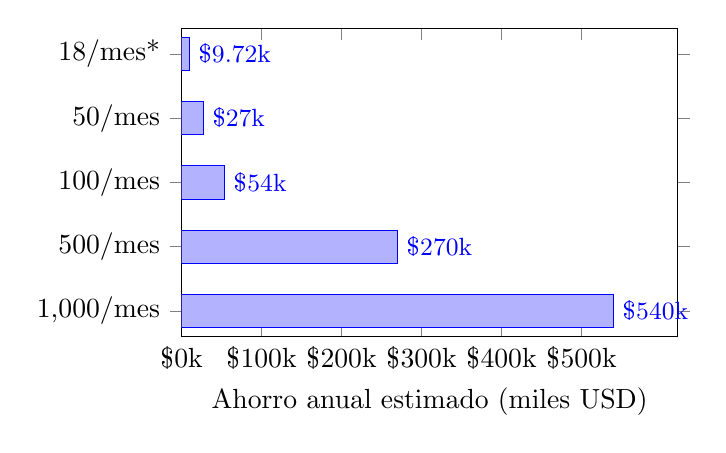
\begin{tikzpicture}
\begin{axis}[
    xbar,
    width=0.65\textwidth,
    height=5.5cm,
    xlabel={Ahorro anual estimado (miles USD)},
    xmin=0, xmax=620,
    xtick={0,100,200,300,400,500},
    xticklabel={\$\pgfmathprintnumber{\tick}k},
    ytick=data,
    yticklabels={18/mes*,50/mes,100/mes,500/mes,{1,000/mes}},
    y dir=reverse,
    bar width=12pt,
    nodes near coords={\$\pgfmathprintnumber{\pgfplotspointmeta}k},
    nodes near coords align={horizontal},
    nodes near coords style={font=\small},
    every axis plot/.append style={fill=teal!60, draw=teal!80!black},
]
\addplot coordinates {(9.72,0) (27,1) (54,2) (270,3) (540,4)};
\end{axis}
\end{tikzpicture}
%\caption{Ahorro anual estimado a USD~30/hora según volumen de incidencias mensuales. *\textit{Fintech} de referencia.}
\caption{Ahorro anual estimado según volumen de incidencias mensuales.}
\label{fig:ahorro_escala}
\end{figure}

Estas cifras representan únicamente el ahorro directo en horas de soporte asociadas a un solo tipo de documento (la carátula bancaria) y no contemplan beneficios adicionales como la reducción de errores propagados a sistemas \textit{downstream}, la mejora en la experiencia del usuario durante el \textit{onboarding}, ni el tiempo ahorrado por los propios usuarios al evitar la transcripción manual de datos. Además, dado que la arquitectura del MVP se basa en extractores configurables, el mismo modelo de ahorro es replicable para cualquier otro tipo de documento que una organización necesite procesar: contratos, comprobantes de domicilio, identificaciones oficiales, pólizas de seguro, entre otros. Cada nuevo extractor configurado representa un proceso operativo adicional que puede beneficiarse de la automatización, multiplicando el impacto económico total. En ese sentido, el valor del sistema no se agota en un único flujo de extracción, sino que escala proporcionalmente con la cantidad de procesos documentales que la organización decida incorporar.


\section{Costos del MVP}

El costo de operar el MVP depende de tres componentes: el procesamiento de documentos mediante la API de Claude, el almacenamiento de archivos en S3 y la infraestructura de servidor y base de datos. A continuación se desglosa cada uno y se presenta un resumen del costo final por solicitud.

\subsection{Claude API}

El costo variable principal del MVP corresponde al uso de la API de Claude, específicamente del modelo \texttt{claude-haiku-4-5-20251001}. Este servicio se emplea tanto para la extracción de información desde documentos como para funciones auxiliares asociadas a la configuración de extractores. Su costo depende del volumen de \textit{tokens} de entrada y salida procesados en cada llamada, como se detalla en la Tabla \ref{tab:claude_api_costos}.
\begin{table}[H]
\centering
\resizebox{0.8\textwidth}{!}{%
\begin{tabular}{lcc}
\toprule
\textbf{Concepto} & \textbf{Detalle} & \textbf{Costo estimado} \\
\midrule
Input tokens & USD 1.00 / millón de tokens & -- \\
Output tokens & USD 5.00 / millón de tokens & -- \\
Imagen (JPG/PNG) & 2 llamadas: orientación + extracción & USD 0.005 \\
PDF chico (1--2 páginas) & 1 llamada, \textasciitilde 3{,}300 input tokens & USD 0.004 \\
PDF mediano (10 páginas) & 1 llamada, \textasciitilde 15{,}300 input tokens & USD 0.016 \\
PDF grande (50 páginas) & 1 llamada, \textasciitilde 75{,}300 input tokens & USD 0.077 \\
PDF máximo (100 páginas) & 1 llamada, \textasciitilde 150{,}300 input tokens & USD 0.150 \\
Generar \textit{schema} & costo one-time por extractor & USD 0.003 \\
Generar \textit{prompt} & costo one-time por extractor & USD 0.003 \\
Refinar \textit{prompt} & costo one-time por extractor & USD 0.004 \\
\bottomrule
\end{tabular}
}
\caption{Costos de procesamiento con Claude API}
\label{tab:claude_api_costos}
\end{table}
En el caso de imágenes, el flujo contempla dos llamadas al modelo: una para verificar la orientación del archivo y otra para realizar la extracción. En el caso de los documentos PDF, Claude procesa cada página como representación visual, con un consumo aproximado de 1{,}500 \textit{tokens} por página, realizando una sola llamada por documento. 

\subsection{S3 Storage}

El almacenamiento de archivos se realiza mediante el servicio de \textit{storage buckets} de Railway, compatible con el protocolo S3, que actualmente se encuentra incluido dentro del \textit{free tier} de la plataforma. En la fase actual del MVP, este componente no representa un costo significativo dentro de la operación. Sin embargo, para tener una referencia de escalamiento, se consideran los costos unitarios mostrados en la Tabla \ref{tab:tigris_storage_costos}. Estos valores muestran que el almacenamiento tiene un impacto marginal frente al costo del procesamiento de documentos, por lo que no constituye el componente central del costo del producto.

\begin{table}[H]
\centering
\resizebox{0.6\textwidth}{!}{%
\begin{tabular}{l c}
\toprule
\textbf{Concepto} & \textbf{Costo} \\
\midrule
PUT (upload) & USD 0.000005 / request \\
GET (download) & USD 0.0000004 / request \\
Almacenamiento & USD 0.023 / GB / mes \\
Total por request & $<$ USD 0.001 \\
Archivo de 20MB almacenado & USD 0.0005 / mes \\
\bottomrule
\end{tabular}
}
\caption{Costos de referencia para almacenamiento S3 en Railway}
\label{tab:tigris_storage_costos}
\end{table}



\subsection{Infraestructura}

La arquitectura del sistema se despliega actualmente sobre Railway, para el \textit{backend} y la base de datos PostgreSQL, y sobre Vercel, para el \textit{frontend}. Durante la etapa inicial del MVP, ambos servicios operan bajo esquemas gratuitos, lo que reduce el costo de validación temprana. No obstante, una vez superados los límites del \textit{free tier}, comienzan a aparecer costos mensuales de infraestructura, cuyo impacto unitario depende del volumen de solicitudes procesadas. La Tabla \ref{tab:infraestructura_costos} evidencia que, al superar la etapa de validación inicial, el producto incorpora un costo fijo mensual asociado al sostenimiento de su arquitectura. Sin embargo, este costo puede prorratearse según el volumen de solicitudes, de modo que su impacto unitario disminuye conforme aumenta el uso del sistema.


\begin{table}[H]
\centering
\resizebox{0.9\textwidth}{!}{%
\begin{tabular}{l c c c}
\toprule
\textbf{Servicio} & \textbf{Costo mensual estimado} & \textbf{A 1{,}000 req/mes} & \textbf{A 10{,}000 req/mes} \\
\midrule
Railway (\textit{backend} + DB) & USD 5--20 / mes & USD 0.02 / req & USD 0.002 / req \\
Vercel (\textit{frontend}) & USD 0--20 / mes & USD 0.02 / req & USD 0.002 / req \\
Total infraestructura & USD 10--40 / mes & USD 0.04 / req & USD 0.004 / req \\
\bottomrule
\end{tabular}
}
\caption{Costos estimados de infraestructura post free-tier}
\label{tab:infraestructura_costos}
\end{table}



\subsection{Resumen de costos finales}

Es posible consolidar el costo final por solicitud en dos escenarios, como muestra la Tabla \ref{tab:resumen_costos_finales}: la fase actual, en la que solo se incurre en costos de procesamiento mediante Claude API, y una fase futura, en la que además se incorpora el costo prorrateado de infraestructura.

\begin{table}[H]
\centering
\resizebox{0.6\textwidth}{!}{%
\begin{tabular}{l c c}
\toprule
\textbf{Escenario} & \textbf{Fase actual} & \textbf{Fase futura} \\
\midrule
Imagen simple & USD 0.005 & USD 0.045 \\
PDF de 1--2 páginas & USD 0.004 & USD 0.044 \\
PDF de 10 páginas & USD 0.016 & USD 0.056 \\
PDF de 50 páginas & USD 0.077 & USD 0.117 \\
PDF de 100 páginas (\textasciitilde 20MB) & USD 0.150 & USD 0.190 \\
\bottomrule
\end{tabular}
}
\caption{Resumen de costos finales por solicitud}
\label{tab:resumen_costos_finales}
\end{table}